\section{Layers}
\subsection{Physical}
  \begin{frame}
    \frametitle{Aims}
      \begin{itemize}
        \item Interface data link layer,\pause
        \item (De)Encode,\pause
        \item Transmit: 1 after 0 (after 0 or 1, after 0... or 1)
      \end{itemize}
  \end{frame}
  \begin{frame}
    \frametitle{Hardware medium}
      \begin{itemize}
        \item IEEE 802.3 (a.k.a. Ethernet): $<$100Gbit/s \pause
        \item IEEE 802.11 (a.k.a. Wi-Fi): $<$50 Mbit/s (802.11ad goes up to 6.75 Gbit/s) \pause
        \item IEEE 802.15.1 (a.k.a. Bluetooth): $<$1 Mbit/s \pause
        \item IEEE 802.15.4 (a.k.a. ZigBee): $<$250 kbit/s \pause
        \item IEEE 802.16 (a.k.a. Wi-Max): $<$40 Mbit/s \pause
        \item IEEE 1394 (a.k.a. Firewire): $<$3200 Mbit/s \pause
        \item USB, serial port such as RS-232...
      \end{itemize}
  \end{frame}
  \begin{frame}
    \frametitle{Hardware medium: IEEE 802.3 (Ethernet)}
    \begin{figure}[t]
      \centering
      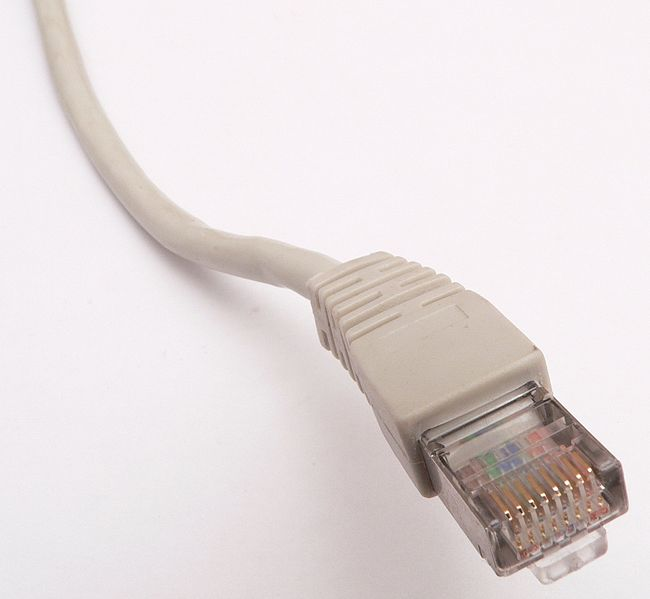
\includegraphics[height=5cm]{./imgs/rj45.jpg}
      \caption{\color{blue}\href{https://en.wikipedia.org/wiki/File:Ethernet_RJ45_connector_p1160054.jpg}{RJ45 connector}}
      \label{fig:rj45}
    \end{figure}
  \end{frame}
  \begin{frame}
    \frametitle{Hardware medium: IEEE 802.15.1 (Bluetooth)}
    \begin{figure}[t]
      \centering
      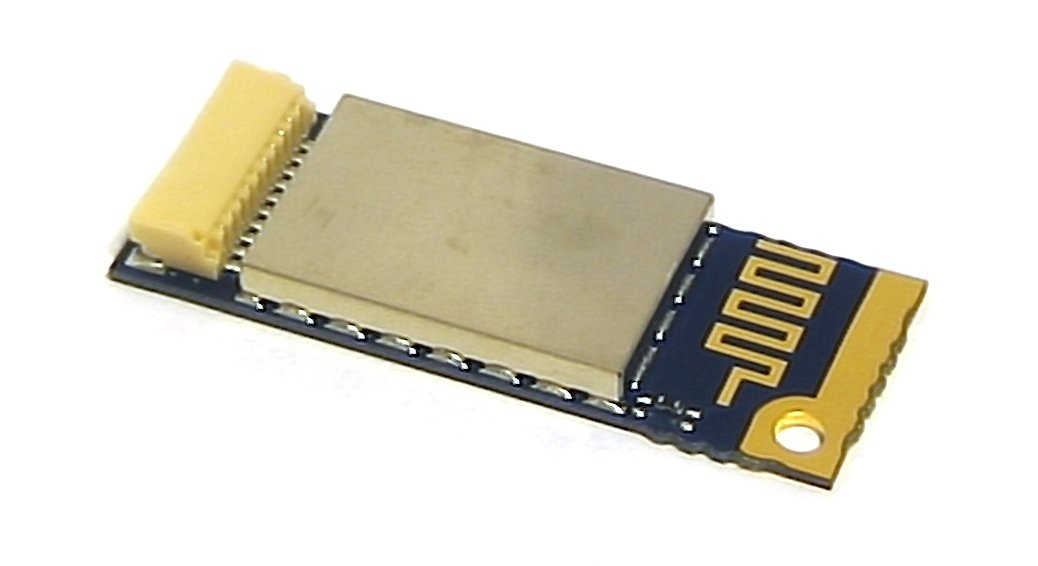
\includegraphics[height=5cm]{./imgs/bluetooth_card}
      \caption{\color{blue}\href{https://upload.wikimedia.org/wikipedia/commons/2/28/DELL_TrueMobile_350_Bluetooth_card.jpg}{Bluetooth card}}
      \label{fig:bluetooth_card}
    \end{figure}
  \end{frame}
  \begin{frame}
    \frametitle{Hardware medium: IEEE 802.15.4 (ZigBee)}
    \begin{figure}[t]
      \centering
      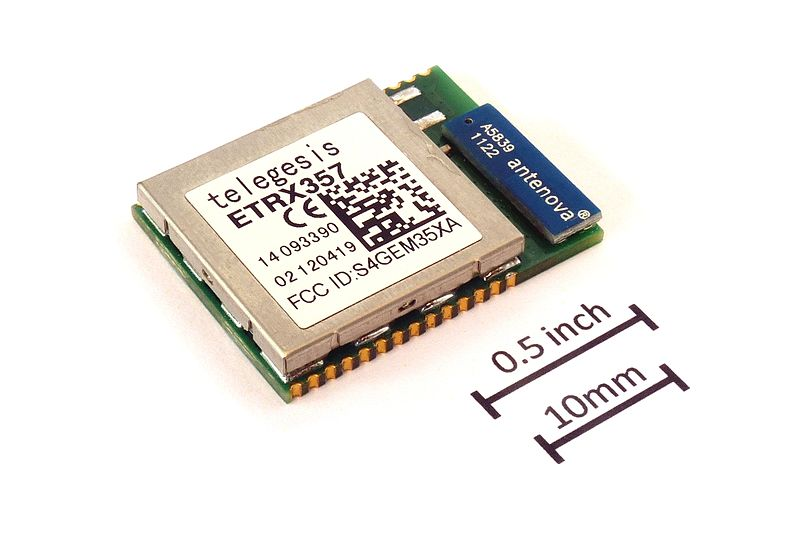
\includegraphics[height=5cm]{./imgs/zigbee.jpg}
      \caption{\color{blue}\href{https://upload.wikimedia.org/wikipedia/commons/thumb/2/29/ETRX357_ZigBee_module_with_size_ref.JPG/800px-ETRX357_ZigBee_module_with_size_ref.JPG}{ZigBee card}}
      \label{fig:ZigBee}
    \end{figure}
  \end{frame}
  \begin{frame}
    \frametitle{Hardware medium: IEEE 802.16 (Wi-Max)}
    \begin{figure}[t]
      \centering
      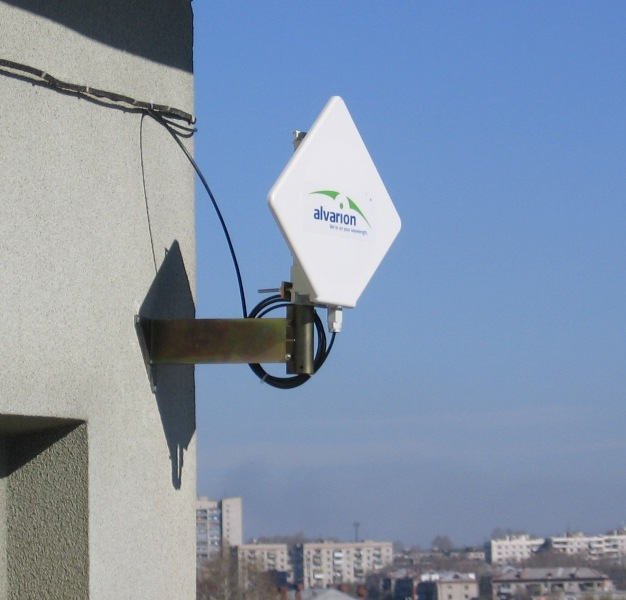
\includegraphics[height=5cm]{./imgs/Wi-Max.jpg}
      \caption{\color{blue}\href{https://upload.wikimedia.org/wikipedia/commons/d/db/Alvarion_CPE.jpg}{Wi-Max antenna}}
      \label{fig:Wi-Max_antenna}
    \end{figure}
  \end{frame}
  \begin{frame}
    \frametitle{Hardware medium: IEEE 1394 (Firewire)}
    \begin{figure}[t]
      \centering
      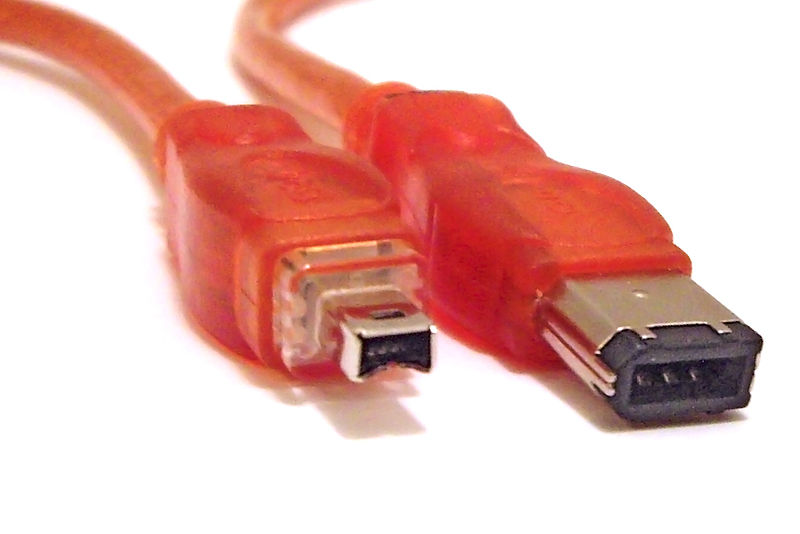
\includegraphics[height=5cm]{./imgs/firewire.jpg}
      \caption{\color{blue}\href{https://upload.wikimedia.org/wikipedia/commons/thumb/f/f7/FireWire_cables.jpg/800px-FireWire_cables.jpg}{Firewire connector}}
      \label{fig:firewire}
    \end{figure}
  \end{frame}
  \begin{frame}
    \frametitle{Encoding}
      \begin{itemize}
        \item \textbf{MLT3 (Multi-Level Transmit):} state change for 1s over 3 levels, stay in the same state for 0s \pause
        \item \textbf{AMI (Alternate Mark Inversion):} state 0 for 0s, state +/-1 for 1s \pause
        \item \textbf{Manchester:} voltage transition (rising/falling edge mean 1/0) \pause
        \item \textbf{BMC (Biphase Mark Code):} change its state for 1s, stay on the same state for 0s \pause
        \item and so on...
      \end{itemize}
  \end{frame}
  \begin{frame}
    \frametitle{Encoding: Multi-Level Transmit}
    \begin{figure}[t]
      \centering
      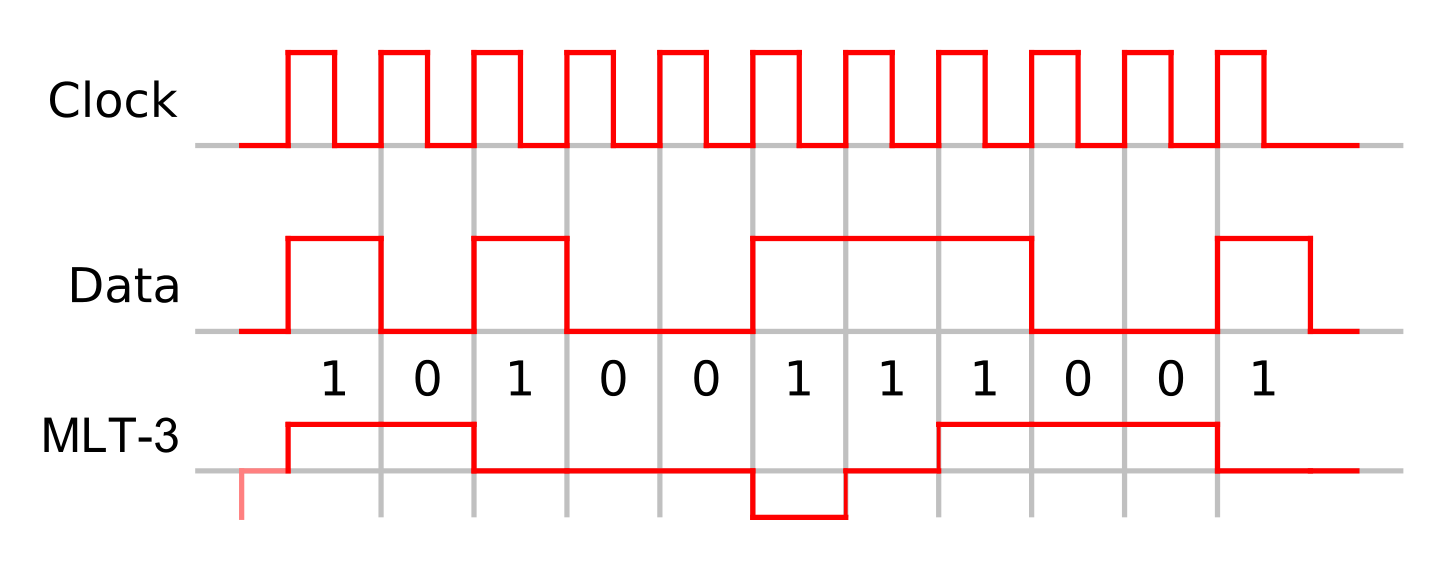
\includegraphics[height=3cm]{./imgs/mlt3.png}
      \caption{\color{blue}\href{https://upload.wikimedia.org/wikipedia/commons/thumb/b/b4/MLT3encoding.svg/1456px-MLT3encoding.svg.png}{Multi-Level Transmit}}
      \label{fig:mlt3}
    \end{figure}
  \end{frame}
  \begin{frame}
    \frametitle{Encoding: Alternate Mark Inversion}
    \begin{figure}[t]
      \centering
      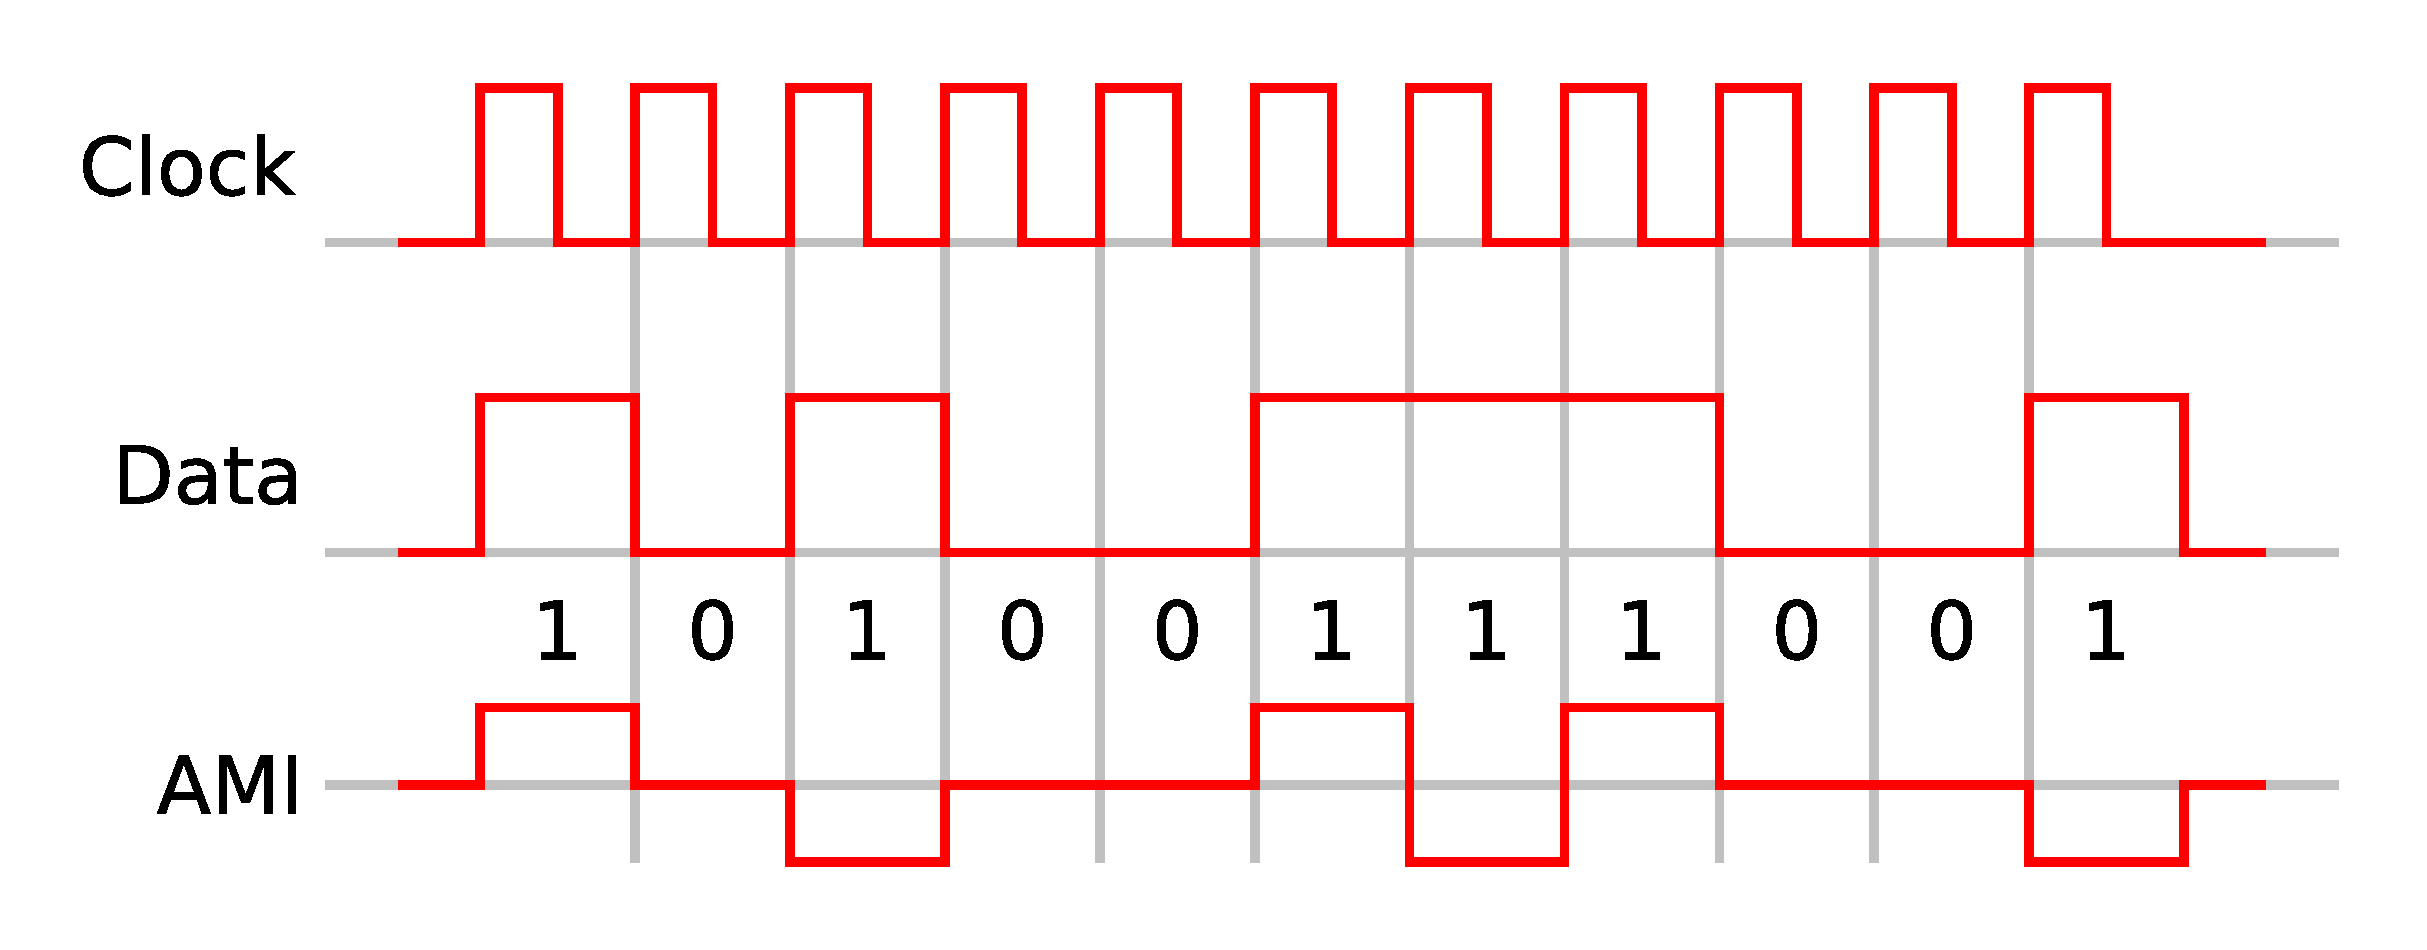
\includegraphics[height=3cm]{./imgs/ami.pdf}
      \caption{\color{blue}\href{https://upload.wikimedia.org/wikipedia/commons/b/b6/Ami_encoding.svg}{Alternate Mark Inversion}}
      \label{fig:ami}
    \end{figure}
  \end{frame}
  \begin{frame}
    \frametitle{Encoding: Manchester}
    \begin{figure}[t]
      \centering
      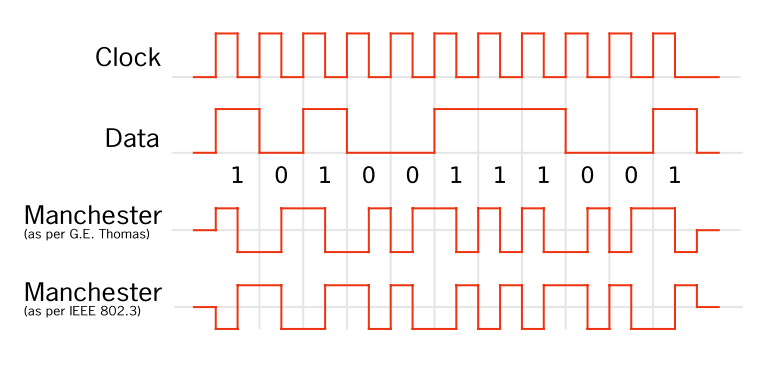
\includegraphics[height=3cm]{./imgs/manchester.png}
      \caption{\color{blue}\href{https://upload.wikimedia.org/wikipedia/commons/thumb/9/90/Manchester_encoding_both_conventions.svg/771px-Manchester_encoding_both_conventions.svg.png}{Manchester}}
      \label{fig:manchester}
    \end{figure}
  \end{frame}
  \begin{frame}
    \frametitle{Encoding: Biphase Mark Code}
    \begin{figure}[t]
      \centering
      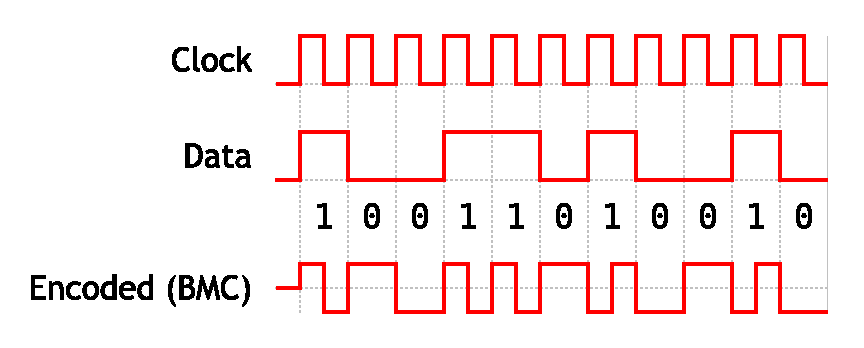
\includegraphics[height=3cm]{./imgs/bmc.pdf}
      \caption{\color{blue}\href{https://upload.wikimedia.org/wikipedia/commons/c/cb/Biphase_Mark_Code.svg}{Biphase Mark Code}}
      \label{fig:bmc}
    \end{figure}
  \end{frame}
  \begin{frame}
    \frametitle{Transmitting}
    \begin{figure}[t]
      \centering
      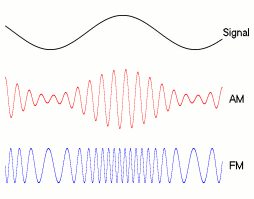
\includegraphics[height=5cm]{./imgs/modulation.png}
      \caption{\color{blue}\href{https://upload.wikimedia.org/wikipedia/commons/a/a4/Amfm3-en-de.gif}{Amplitude and phase modulation}}
      \label{fig:modulation}
    \end{figure}
  \end{frame}
  \begin{frame}
    \frametitle{Error detection}
      \begin{itemize}
        \item Repetition (hum...) \pause
        \item Parity (XOR) \pause
        \item Checksum \pause
        \item CRC (Cyclic redundancy check): with a polynomial divison \pause
        \item Hash \pause
        \item and so on...
      \end{itemize}
  \end{frame}
  \begin{frame}
    \frametitle{Error correcting}
      \begin{itemize}
        \item Repetition (again) \pause
        \item Hamming \pause
        \item MDPC (Multidimensional parity-check code)
      \end{itemize}
  \end{frame}

  \begin{frame}
    \frametitle{Correction: MDPC}
    Raw data to send: 0x01 02 03 04
      \begin{figure}[h]
      \centering
      \begin{tabular}{cc|c}
        0x01 & 0x02 & 0x03 \\
        0x03 & 0x04 & 0x07 \\ \hline
        0x04 & 0x06 &
      \end{tabular}
      \caption{Data received with MDPC}
      \label{fig:ami}
    \end{figure}
  Data sent (with MDPC): 0x01 02 03 03 04 07 04 06
  \end{frame}
\subsection{Data Link}
  \begin{frame}
    \frametitle{Aims}
      \begin{itemize}
        \item Interface network layer,\pause
        \item Delivery to unique(?) hardware addresses,\pause
        \item Framing,\pause
        \item Data transfer
      \end{itemize}
  \end{frame}
  \begin{frame}
    \frametitle{Layer composition (of its two sublayers)}
      \begin{enumerate}
        \item Logical Link Control (LLC):
          \begin{itemize}
            \item end to end flow control
            \item end to end error control
            \item (transmitting/receiving) protocols, over MAC sublayer, multiplexing
          \end{itemize}\pause
        \item Media Access Control (MAC):
          \begin{itemize}
            \item physical (hardware) addressing
            \item collision detection and retransmission
            \item data packet scheduling (and queuing)
            \item QoS
            \item VLAN
          \end{itemize}\pause
      \end{enumerate}
  \end{frame}
  \begin{frame}
    \frametitle{Carrier Sense Multiple Access with Collision Avoidance}
    \begin{figure}[t]
      \centering
      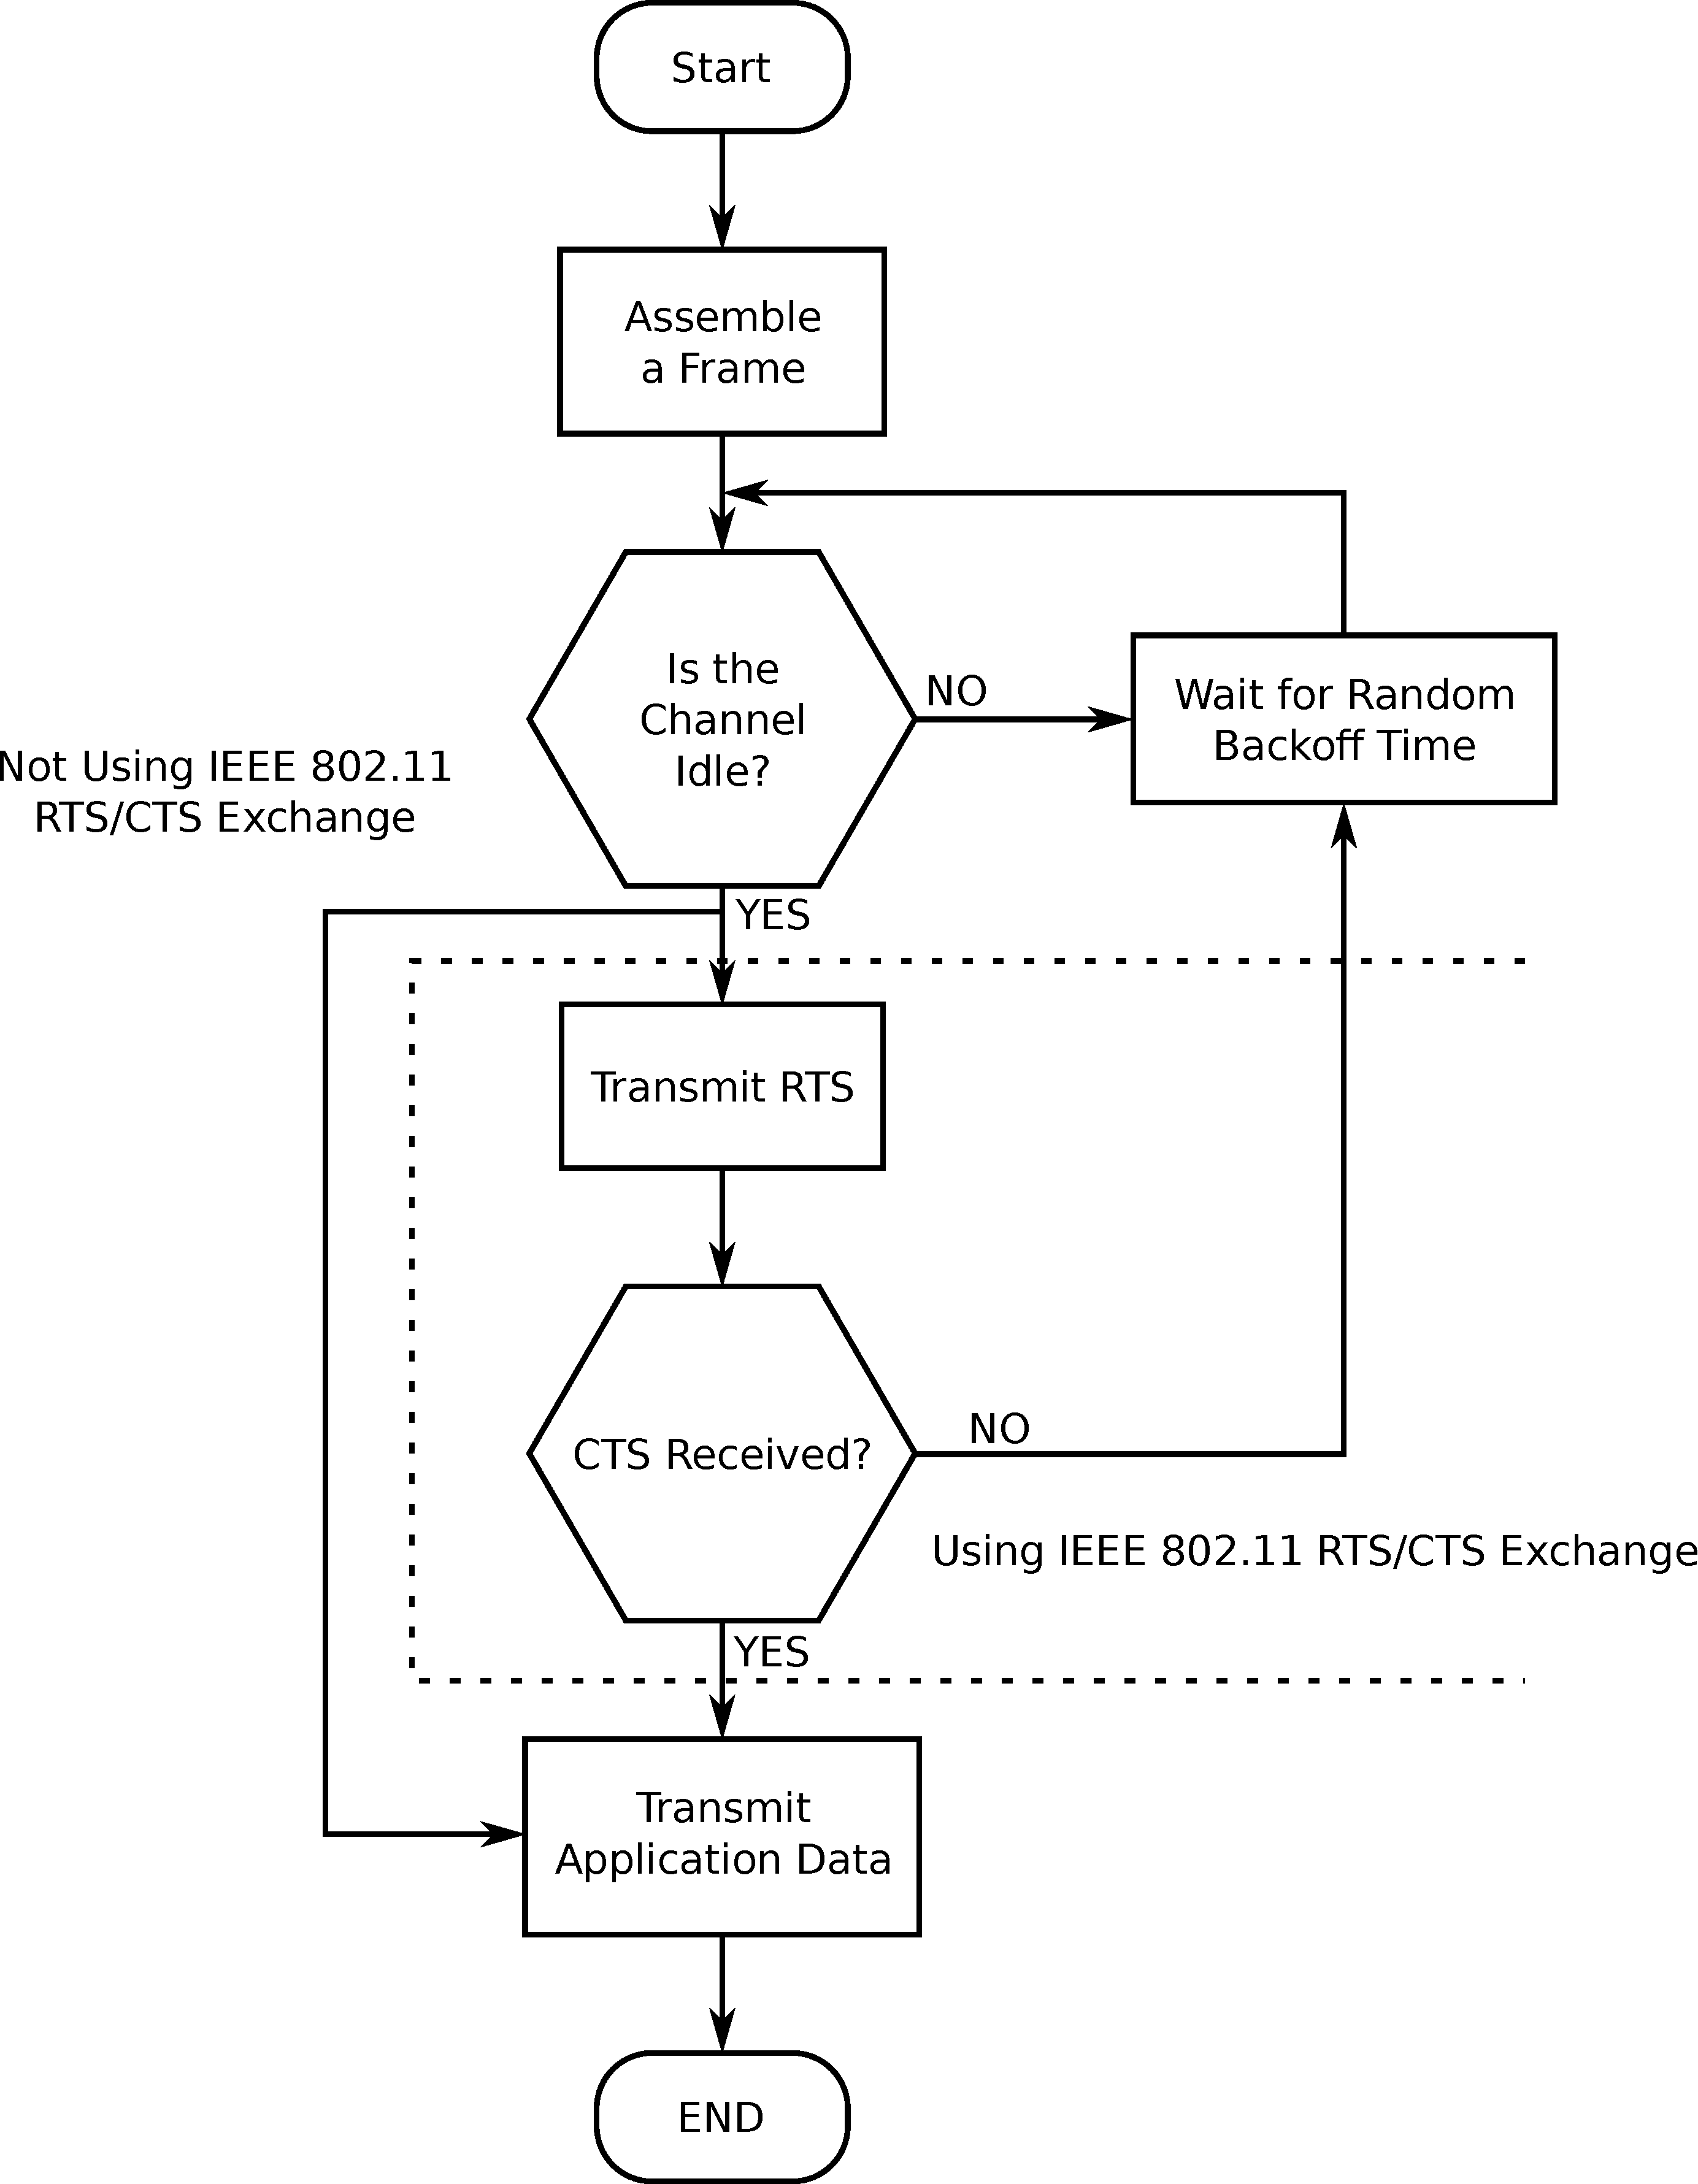
\includegraphics[height=6cm]{./imgs/csma_ca.pdf}
      \caption{\color{blue}\href{https://en.wikipedia.org/wiki/File:Csma_ca.svg}{CSMA CA}}
      \label{fig:csma_ca}
    \end{figure}
    \end{frame}
  \begin{frame}
    \frametitle{Layer 2 Ethernet packet}
      \begin{figure}[h]
      \centering
      \begin{tabular}{|c|c|c|c|c|c|c|c|c|}
        \hline
        \multicolumn{3}{|c|}{MAC dest. (\color{blue}6\color{black})} & \multicolumn{3}{|c|}{MAC src. (\color{blue}6\color{black})} & \multicolumn{2}{|c|}{\color{brown}VLAN tag* (\color{blue}4\color{brown})\color{black}} & Ethertype (\color{blue}2\color{black}) \\ \hline
        \multicolumn{6}{|c|}{Payload (\color{blue}42-1500\color{black})} & \multicolumn{3}{|c|}{Frame check sequence (\color{blue}4\color{black})}\\ \hline
      \end{tabular}
      \caption{Layer 2 Ethernet packet}
      \label{fig:eth_packet}
    \end{figure}
    \hfill \color{brown}optional\color{black}, Content (\color{blue}size in bytes\color{black})
    \begin{figure}[h]
      \centering
      \begin{tabular}{|c|c|}
        \hline
        \textbf{Ethertype 0x} & \textbf{Protocol} \\ \hline
        0800 & IPv4 \\ \hline
        0806 & ARP \\ \hline
        0842 & Wake-on-LAN \\ \hline
        86dd & IPv6 \\ \hline
      \end{tabular}
      \caption{Data received with MDPC}
      \label{fig:eth_type}
    \end{figure}
  \end{frame}


  \begin{frame}
    \frametitle{ARP example}
      \begin{figure}
      \centering
      \resizebox{11.5cm}{!} {
        \begin{tabular}{lccccccccccccccccc}
          \textbf{0000} & ff & ff & ff & ff & ff & ff & fa & ba & ba & 00 & ab & ab & af & 08 & 06 & 00 & 01 \\
          \textbf{0010} & 08 & 00 & 06 & 04 & 00 & 01 & fa & ba & ba & 00 & ab & ab & af & ac & 11 & 22 & 37 \\
          \textbf{0020} & 00 & 00 & 00 & 00 & 00 & 00 & ac & 11 & 00 & f9 & 00 & 00 & 00 & 00 & 00 & 00 & 00 \\
          \textbf{0030} & 00 & 00 & 00 & 00 & 00 & 00 & 00 & 00 & 00 & 00 & 00 & 00 \\
        \end{tabular}
      }
      \caption{Layer 2 Ethernet packet}
      \label{fig:arp_packet_ex}
    \end{figure}
  \end{frame}

  \begin{frame}
    \frametitle{ARP example}
      \begin{figure}
      \centering
      \resizebox{11.5cm}{!} {
        \begin{tabular}{lccccccccccccccccc}
          \textbf{0000} & \color{red}ff & \color{red}ff & \color{red}ff & \color{red}ff & \color{red}ff & \color{red}ff & \color{Marroon}fa & \color{Marroon}ba & \color{Marroon}ba & \color{Marroon}00 & \color{Marroon}ab & \color{Marroon}ab & \color{Marroon}af & \color{blue}08 & \color{blue}06 & \color{magenta}00 & \color{magenta}01 \\
          \textbf{0010} & \color{OliveGreen}08 & \color{OliveGreen}00 & \color{gray}06 & \color{gray}04 & \color{gray}00 & \color{gray}01 & \color{Marroon}fa & \color{Marroon}ba & \color{Marroon}ba & \color{Marroon}00 & \color{Marroon}ab & \color{Marroon}ab & \color{Marroon}af & \color{brown}ac & \color{brown}11 & \color{brown}22 & \color{brown}37 \\
          \textbf{0020} & \color{red}00 & \color{red}00 & \color{red}00 & \color{red}00 & \color{red}00 & \color{red}00 & \color{orange}ac & \color{orange}11 & \color{orange}00 & \color{orange}f9 & 00 & 00 & 00 & 00 & 00 & 00 & 00 \\
          \textbf{0030} & 00 & 00 & 00 & 00 & 00 & 00 & 00 & 00 & 00 & 00 & 00 & 00 \\
        \end{tabular}
      }
      \caption{Layer 2 Ethernet packet}
      \label{fig:arp_packet_ex}
    \end{figure}
    \color{red}MAC address destination \color{Marroon}MAC address source \color{blue}Ethertype \color{magenta}Hardware type \color{OliveGreen}Protocol type \color{brown} IP address source \color{orange} IP address destination
  \end{frame}


  \subsection{Network}
  \begin{frame}
    \frametitle{Course details}
  \end{frame}
\subsection{Transport}
  \begin{frame}
    \frametitle{Course details}
  \end{frame}
